\chapter{Dominating Set}

Rishank was pleased to see Ajur and Jura who were on the lookout for a water fountain, and told them that placing a water fountain is an interesting graph theoretic problem. Rishnak started with a definition of a Dominating Set. A dominating set of a graph $G=(V,E)$ is a subset of vertices, $D$, such that every vertex in $V-D$ (that is a vertex $x~in ~V $ but $\notin~ D$) is adjacent to some vertex in $D$. Rishnak realized that his definition was a bit dense and so he drew the followig graph and its dominating set Figure \ref{18g1}.
\begin{figure}
\begin{center}
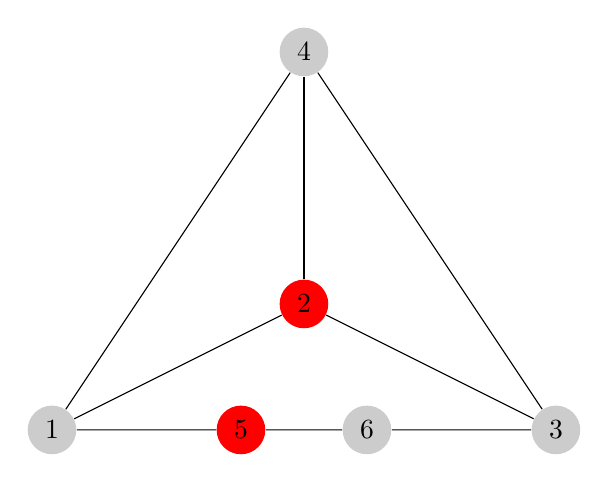
\begin{tikzpicture}
  [scale=.8,auto=left,every node/.style={circle,fill=black!20}]
  \node (n1) at (-1,7) {1};
  \node (n2)[fill=red] at (3,9)  {2};
  \node (n3) at (7,7)  {3};
  \node (n4) at (3,13)  {4};
  \node (n5)[fill=red] at (2,7) {5};
  \node (n6) at (4,7) {6};
 \foreach \from/\to in {n1/n2,n2/n3,n2/n4,n1/n4,n3/n4,n1/n5,n5/n6,n6/n3}
    \draw (\from) -- (\to);
\end{tikzpicture}
\caption{ Dominating vertices are colored red. Every vertex not colored red is adjacent to one of the red vertices}\label{18g1}
\end{center}
\end{figure}

Rishnak added that Dominating set and vertex cover may seem similar, but they are not. In a vertex cover, every edge is incident on one of the vertices in the vertex cover. In general, we want to find the minimum dominating set. Ajur saw the connection between placing a water fountain and the dominating set.

Here is a map of Royt shown in Figure \ref{18g2}. Rishnak asked Ajur where will he place the water fountains with a condition that every junction/corner has either a water fountain or adjacent to a water fountain (we assume people walk less than two edges to reach a water fountain)
\begin{figure}
\begin{center}

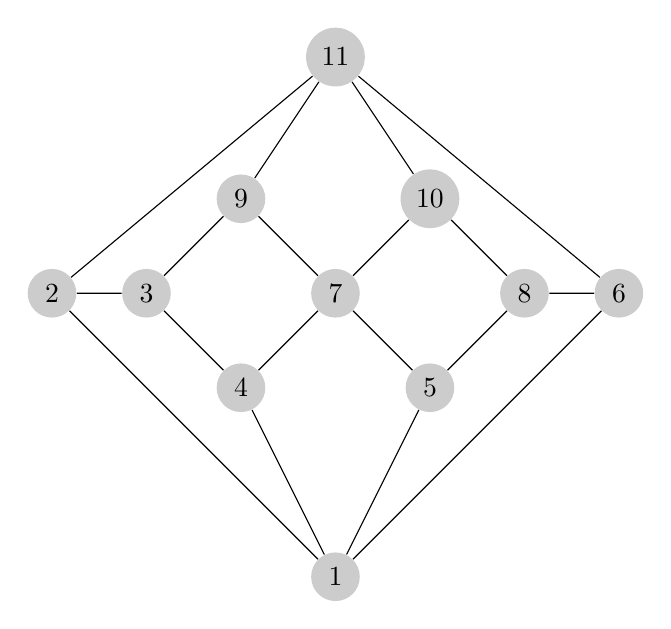
\begin{tikzpicture}
  [scale=.6,auto=left,every node/.style={circle,fill=black!20}]
  \node (n1) at (6,-3) {1};
  \node (n2) at (0,3)  {2};
  \node (n3) at (2,3)  {3};
  \node (n4) at (4,1) {4};
  \node (n5) at (8,1)  {5};
  \node (n6) at (12,3)  {6};
  \node (n7) at (6,3)  {7};
 \node (n8) at (10,3) {8};
  \node (n9) at (4,5)  {9};
  \node (n10) at (8,5)  {10};
  \node (n11) at (6,8)  {11}; 

  \foreach \from/\to in {n1/n2,n1/n4,n1/n5,n1/n6,n2/n3,n2/n11,n3/n4,n3/n9,n4/n7,n5/n7,n5/n8,n6/n8,n6/n11,n7/n9,n7/n10,n8/n10,n9/n11,n10/n11}
    \draw (\from) -- (\to);

\end{tikzpicture}
\caption{Street Map of Royt. Where to place the water fountains}\label{18g2}
\end{center}
\end{figure}

Ajur felt challenged and he had to think hard. He knew that placing minimum number of water fountains is the same as finding the dominating set. He placed water fountains in vertices 2, 6 and 7 as shown in Figure \ref{18g3}.

\begin{figure}
\begin{center}

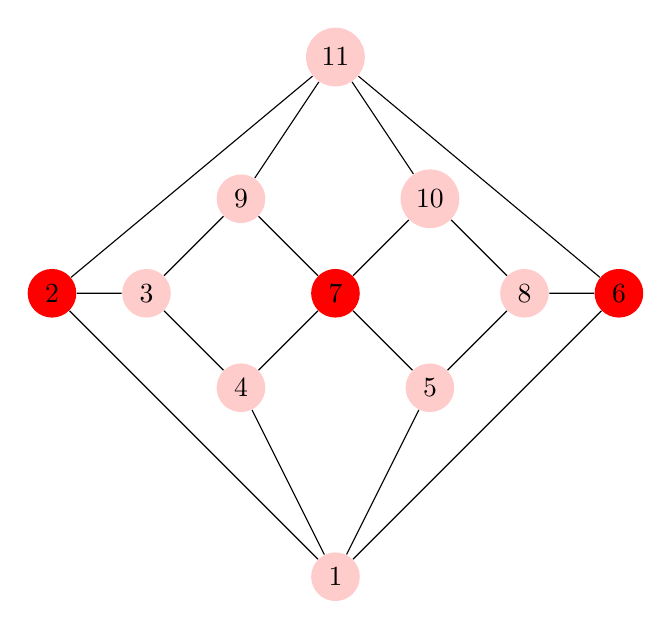
\begin{tikzpicture}
  [scale=.6,auto=left,every node/.style={circle,fill=red!20}]
  \node (n1) at (6,-3) {1};
  \node (n2)[fill=red] at (0,3)  {2};
  \node (n3) at (2,3)  {3};
  \node (n4) at (4,1) {4};
  \node (n5) at (8,1)  {5};
  \node (n6)[fill=red] at (12,3)  {6};
  \node (n7)[fill=red] at (6,3)  {7};
 \node (n8) at (10,3) {8};
  \node (n9) at (4,5)  {9};
  \node (n10) at (8,5)  {10};
  \node (n11) at (6,8)  {11}; 

  \foreach \from/\to in {n1/n2,n1/n4,n1/n5,n1/n6,n2/n3,n2/n11,n3/n4,n3/n9,n4/n7,n5/n7,n5/n8,n6/n8,n6/n11,n7/n9,n7/n10,n8/n10,n9/n11,n10/n11}
    \draw (\from) -- (\to);

\end{tikzpicture}
\caption{Water Fountains are placed in vertices 2, 6 and 7 }\label{18g3}
\end{center}
\end{figure}

Rishnak then introduced the Total dominating set problem, a variation of a dominating set problem. A total dominating set $TD$ of a graph $G=(V,E)$ such that every vertex $v~\in~V$ is adjacent to some vertex in $TD$. For example the dominating set $\{2,6,7\}$ shown in Figure \ref{18g3} is not a Total dominating set. Ajur answered that as vertex 2 is not adjacent to any of $\{2,6,7\}$.\footnote{A vertex is not adjacent to itself.} Rishnak asked Ajur what the total dominating set for Figure \ref{18g2} is.

Ajur had to think hard and responded that vertices 3, 4, 7, 8, 10 form a total dominating set. He was not sure whether that was the minimum total dominating set. Rishnak said that if one did not include vertex 7, then it would still be total dominating set and drew the graph in Figure \ref{18g4}.

\begin{figure}
\begin{center}

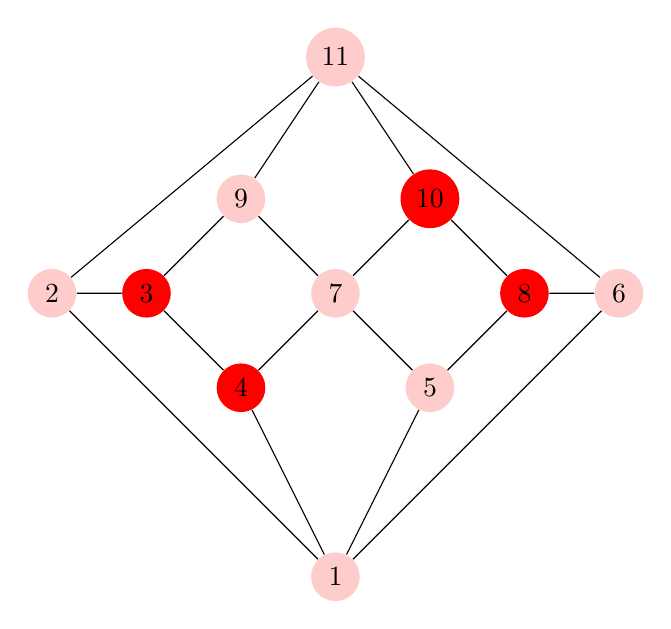
\begin{tikzpicture}
  [scale=.6,auto=left,every node/.style={circle,fill=red!20}]
  \node (n1) at (6,-3) {1};
  \node (n2) at (0,3)  {2};
  \node (n3)[fill=red] at (2,3)  {3};
  \node (n4)[fill=red] at (4,1) {4};
  \node (n5) at (8,1)  {5};
  \node (n6) at (12,3)  {6};
  \node (n7) at (6,3)  {7};
 \node (n8) [fill=red]at (10,3) {8};
  \node (n9) at (4,5)  {9};
  \node (n10)[fill=red] at (8,5)  {10};
  \node (n11) at (6,8)  {11}; 

  \foreach \from/\to in {n1/n2,n1/n4,n1/n5,n1/n6,n2/n3,n2/n11,n3/n4,n3/n9,n4/n7,n5/n7,n5/n8,n6/n8,n6/n11,n7/n9,n7/n10,n8/n10,n9/n11,n10/n11}
    \draw (\from) -- (\to);

\end{tikzpicture}
\caption{Total Dominating set of vertices 3, 4, 8 and 10 (filled red) }\label{18g4}
\end{center}
\end{figure}

By this time, they did find the water fountain. Ajur and Jura went to play and Rishnak went back to chatting with his ghost friends.